%!tex program = lualatex
\documentclass{ctexart}
\usepackage{amsmath, amssymb}
\usepackage{xcolor}
\usepackage{pgfplots}
\pgfplotsset{compat=1.18}
\ctexset{
  section/name = {问题},
  section/nameformat += {\sffamily},
  section/numberformat += {\color{magenta}\Huge}
}
%%%%%%%%%%%%%%%%%%%%%%%%%%%%%%%%%%%%%%%%%%%%%%%%%%%%%%%%%%%%%%%%%%%%%%%%%%%%%%%
\usepackage[most]{tcolorbox}
\usetikzlibrary{arrows.meta}
%%%%%%%%%%%%%%%%%%%%%%%%%%%%%%%%%%%%%%%%%%%%%%%%%%%%%%%%%%%%%%%%%%%%%%%%%%%%%%%
\usepackage{algorithm}
\usepackage{algpseudocodex}
\usepackage{caption}
\captionsetup[algorithm]{name={算法}}
%%%%%%%%%%%%%%%%%%%%%%%%%%%%%%%%%%%%%%%%%%%%%%%%%%%%%%%%%%%%%%%%%%%%%%%%%%%%%%%
\usepackage{silence}
\WarningFilter{latexfont}{Font shape}
\WarningFilter{latexfont}{Size substitutions}
\WarningFilter{latexfont}{Some font}
\hfuzz=15pt
%%%%%%%%%%%%%%%%%%%%%%%%%%%%%%%%%%%%%%%%%%%%%%%%%%%%%%%%%%%%%%%%%%%%%%%%%%%%%%%
\usepackage{hyperref}
\hypersetup{
  colorlinks = true,
  urlcolor = magenta,
  linkcolor = cyan
}
%%%%%%%%%%%%%%%%%%%%%%%%%%%%%%%%%%%%%%%%%%%%%%%%%%%%%%%%%%%%%%%%%%%%%%%%%%%%%%%
\newcommand{\red}[1]{\textcolor{red}{#1}}
%%%%%%%%%%%%%%%%%%%%%%%%%%%%%%%%%%%%%%%%%%%%%%%%%%%%%%%%%%%%%%%%%%%%%%%%%%%%%%%
\usepackage{siunitx}
\sisetup{
  group-separator = {,},
}
%%%%%%%%%%%%%%%%%%%%%%%%%%%%%%%%%%%%%%%%%%%%%%%%%%%%%%%%%%%%%%%%%%%%%%%%%%%%%%%
\begin{document}
\section{3或5的倍数}\label{sec:problem01}
\subsection{Problem Description}
\begin{tcolorbox}
	如果我们列出所有小于10的自然数,这些数是3或5的倍数,我们会得到3、5、6和9。它们的和是23。

	请找出所有小于1000的3或5的倍数的和。

	\href{https://projecteuler.net/problem=1}{原问题链接}
\end{tcolorbox}

\subsection{算法}
\begin{algorithm}
	\caption{找到3或5的倍数的和}
	\begin{algorithmic}
		\State 初始化 sum $\gets 0$
		\For{$i = 1$ \to $N-1$}
		\If{$i \mod 3 = 0$ \textbf{or} $i \mod 5 = 0$}
		\State sum $\gets$ sum + $i$
		\EndIf
		\EndFor
		\Return sum
	\end{algorithmic}
\end{algorithm}
这里面要注意题目中要求的是小于上限。

\subsection{答案}
233168

\chapter{Even Fibonacci numbers}
\section{Description}
Each new term in the Fibonacci sequence is generated by adding the previous two terms. By starting with 1 and 2, the first 10 terms will be:
\[1, 2, 3, 5, 8, 13, 21, 34, 55, 89, \dots\]

By considering the terms in the Fibonacci sequence whose values do not exceed four million, find the sum of the even-valued terms.

\section{Flow Chart}
\begin{center}
	\begin{tikzpicture}[node distance=2cm]
		\node (start) [startstop] {开始};
		\node (input) [io, right of=start, xshift=4cm] {输入一个上限值cap};
		\node (op1) [operation, below of=input] {a = 0; \\
			b = 1\\
			sum = 0;};
		\node (op2) [operation, below of=op1] {c = a + b;\\
			a = b;\\
			b = c;};
		\node (dec1) [decision, below of=op2, yshift=-.5cm] {c \% 2 == 0};
		\node (op3) [operation, below of=dec1, yshift=-.3cm] {sum += c;};
		\node (dec2) [decision, below of=op3] {c < cap};
		\node (output) [io, below of=dec2] {输出答案};
		\node (end) [startstop, left of=output, xshift=-4cm] {结束};

		\draw [arrow] (start) -- (input);
		\draw [arrow] (input) -- (op1);
		\draw [arrow] (op1) -- (op2);
		\draw [arrow] (op2) -- (dec1);
		\draw [arrow] (dec1) -- node[right]{Yes} (op3);
		\draw [arrow] (op3) --  (dec2);
		\draw [arrow] (dec2) -- node[right]{No} (output);
		\draw [arrow] (dec2.west) -| node[above=3cm, xshift=-.5cm] {Yes}([xshift=-2cm]op2.west) --  (op2.west);
		\draw [arrow] (output) --  (end);
	\end{tikzpicture}
	\captionof{figure}{Sum Of Even Fibonacci}
\end{center}

\section{Codes}
\begin{cpp}
	std::vector<int> Solution::fibs(int cap)
	{
		std::vector<int> fb;
		int a = 0, b = 1, c = 1;

		while(c <= cap)
		{
			fb.push_back(c);
			a = b;
			b = c;
			c = a + b;
		}

		return fb;
	}

	long Solution::sum_of_even_fibs(int cap)
	{
		long sum{};
		std::vector<int> fb = fibs(cap);

		for(auto item : fb)
		{
			if(item % 2 == 0) sum += item;
		}

		return sum;
	}
\end{cpp}

\section{最大质因数}
\subsection{问题描述}
\begin{tcolorbox}
	$13195$ 的质因数是 $5, 7, 13$ 和 $29$。

	求数 $600851475143$ 的最大质因数。

	\href{https://projecteuler.net/problem=3}{原题链接}
\end{tcolorbox}

\subsection{算法}
素数的判定是一个经典的算法问题,主要有以下一些常见的算法。这些算法根据使用场景的不同各有优劣。
\subsubsection{试除法}
\begin{algorithm}
	\caption{素数判断}
	\label{IsPrime}
	\begin{algorithmic}[1]
		\Function{IsPrime}{n}
		\State \( r \gets 2 \)
		\While{ \(  r \leqslant \lfloor \sqrt{n} \rfloor \)}
		\If{ \( n \bmod r = 0 \)}
		\Return false
		\EndIf
		\State \( r \gets r + 1 \)
		\EndWhile
		\Return true
		\EndFunction
	\end{algorithmic}
\end{algorithm}
这个素数判定法也称为试除法,已经比素数的定义做了一点优化。素数的定义是除了能被1和本身整除,这里只试除到 \(
\lfloor\sqrt{n}\rfloor \)。因为如果存在比 \( \lfloor\sqrt{n}\rfloor \)大的因子 \( i \),那么肯定也存在比个小于 \( \lfloor
\sqrt{n} \rfloor \)的因子 \( j \), 使得 \( i \times j = n \),而 \( j \)在之前已经判断过所以	\( i \)就不需要判断了。

\subsubsection{改进试除法}
试除法还可以进一步优化,主要有两点:
\begin{enumerate}
	\item 跳过偶数: 除了2以外,所有的素数都是奇数;
	\item 跳过合数:进一步跳过所有能够被2或者3整除的数,检查从5开始,每次递增6(即检查 \( 6k-1 \text{和} 6k + 1 \))。
\end{enumerate}
\begin{figure}[htbp]
	\centering
	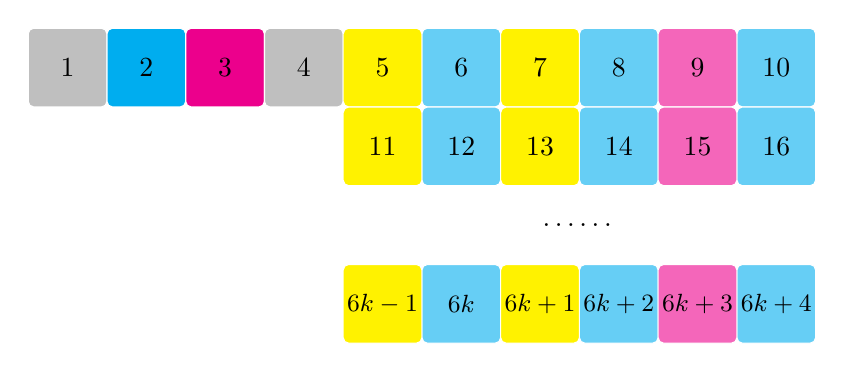
\begin{tikzpicture}[draw=white, rounded corners=2pt]
		\draw[fill=lightgray] (1,0) rectangle node{1}+(1,1);
		\draw[fill=cyan] (2,0) rectangle node{2}+(1,1);
		\draw[fill=magenta] (3,0) rectangle node{3}+(1,1);
		\draw[fill=lightgray] (4,0) rectangle node{4}+(1,1);
		\foreach \x in {6,8,10}
			{
				\draw[fill=cyan!60] (\x, 0) rectangle node{\x} +(1,1) ;
			}
		\draw[fill=yellow] (5,0) rectangle node{5}+(1,1);
		\draw[fill=yellow] (7,0) rectangle node{7}+(1,1);
		\draw[fill=magenta!60] (9,0) rectangle node{9} +(1,1);
		\foreach \x in {6,8,10}
			{
				\draw[fill=cyan!60] (\x, -1) rectangle
				node{\pgfmathparse{int(\x + 6)}\pgfmathresult} +(1,1) ;
			}
		\draw[fill=yellow] (5,-1) rectangle node{11}+(1,1);
		\draw[fill=yellow] (7,-1) rectangle node{13}+(1,1);
		\draw[fill=magenta!60] (9,-1) rectangle node{15} +(1,1);
		\node at (8, -1.5) {$\dots\dots$};
		\foreach \x/\n in {6/$6k$,8/$6k+2$,10/$6k+4$}
			{
				\draw[fill=cyan!60] (\x, -3) rectangle
				node{\small\n} +(1,1) ;
			}
		\draw[fill=yellow] (5,-3) rectangle node{\small$6k-1$}+(1,1);
		\draw[fill=yellow] (7,-3) rectangle node{\small$6k+1$}+(1,1);
		\draw[fill=magenta!60] (9,-3) rectangle node{\small$6k+3$} +(1,1);
	\end{tikzpicture}
	\caption{试除法改进图示}
\end{figure}

\begin{algorithm}[htbp]
	\caption{改进的素数判断}
	\label{algo:IsPrimeImproved}
	\begin{algorithmic}[1]
		\Function{IsPrimeImproved}{n}
		\If{ \( n \leqslant 3 \)}
		\Return \( n > 1 \)
		\EndIf
		\If{ \( n \bmod 2 = 0 \textbf{ or } n \bmod 3 = 0 \)}
		\Return false
		\EndIf
		\State \( r \gets 5 \)
		\While{ \( r^2 \leqslant n \)}
		\If{ \( n \bmod r = 0 \textbf{ or } n \bmod (r + 2) = 0 \)}
		\Return false
		\EndIf
		\State \( r \gets r + 6 \)
		\EndWhile
		\Return true
		\EndFunction
	\end{algorithmic}
\end{algorithm}
这种算法效率比普通的试除法高得多,尤其是当 \( n \) 很大时。

\subsubsection{埃拉托斯特尼筛法}
如果需要判断多个数是否为素数,可以预先生成素数表。这种算法是通过逐步标记合数的方式生成所有不大于某个给定数 \( N \) 的素数表。伪代码如下:
\begin{algorithm}
	\caption{埃拉托斯特尼筛法}
	\label{algo:SieveOfEratosthenes}
	\begin{algorithmic}[1]
		\Function{SieveOfEratosthenes}{N}
		\State 创建布尔数组 \textit{primes},大小为 \( N+1 \),初始全为 \textbf{true}
		\State \( \textit{primes}[0] \gets \textbf{false} \)
		\State \( \textit{primes}[1] \gets \textbf{false} \) \Comment{0 和 1 不是素数}
		\For{ \( p \gets 2 \) \textbf{to} \( \lfloor \sqrt{N} \rfloor \)}
		\If{ \( primes[p] = \textbf{true} \)}
		\For{ \( i \gets p^2 \) to \( N \) by \( p \)}
		\State \( \textit{primes}[i] \gets \textbf{false} \)
		\EndFor
		\EndIf
		\EndFor
		\Return \textit{primes}
		\EndFunction
	\end{algorithmic}
\end{algorithm}

可以看到这种筛法里面有重复的计算,比如8会被4和2都筛一次,如果数值较大的情况下,算力浪费较多。

\subsubsection{欧拉筛法}
欧拉筛法是对埃拉托斯特尼筛法的改进,去除重复筛选的部分。欧拉筛法的关键是每个合数只被最小质因数筛选一次。
伪代码如下:
\begin{algorithm}
	\caption{欧拉筛法}
	\label{algo:SieveOfEuler}
	\begin{algorithmic}[1]
		\Function{SieveOfEuler}{N}
		\State 创建布尔数组 \textit{primeStatus},大小为 \( N+1 \),初始全为 \textbf{true}
		\State \( \textit{primeStatus}[0] \gets \textbf{false} \)
		\State \( \textit{primeStatus}[1] \gets \textbf{false} \) \Comment{0 和 1 不是素数}
		\State 创建数组 \textit{primes}用于存放素数,初始为空
		\For{ \( n \gets 2 \) to \( \lfloor \sqrt{N} \rfloor + 1 \)}
		\If{ \( primeStatus[n] = \textbf{true} \)}
		\State 将 n 推进 primes 数组中
		\EndIf
		\For{每个 \( primes \)中的素数 \( p \)}
		\If{ n \times p > n} \State break \Comment{越界检查}
		\EndIf
		\State \(  {primeStatus[n \times p] \gets \textbf{false}}\)
		\If{ \( p \mid n\)} \Comment{这一步是关键,如果p整除n,则中止循环。比如循环到 \( n=15
		\)时,首先会将30标记为合数,然后是45,但是因为3整除15,所以就中止循环。这样就使得后面的60这些数只被它的最小质因数筛一次。}
		\State break;
		\EndIf
		\EndFor
		\EndFor
		\Return \textit{primes}
		\EndFunction
	\end{algorithmic}
\end{algorithm}

\subsubsection{米勒-拉宾素性测试}
\subsubsection*{米勒-拉宾素性测试的原理}
\begin{enumerate}
	\item 基本概念

	      米勒-拉宾测试是基于以下数学定理:

	      费马小定理(Fermat's Little Theorem):
	      如果 \( p \) 是素数,且 \( a \) 是任意整数且 \( a \) 不被 \( p \) 整除,那么:
	      \[ a^{p-1} \equiv 1 \pmod{p} \]

	      米勒-拉宾测试通过对这个定理进行扩展,来检查一个数是否可能是素数。它是一个概率性算法,意味着测试结果可能存在一定的误差,但通过多次测试,可以使误差变得非常小。
	\item  算法步骤

	      以下是米勒-拉宾素性测试的基本步骤:

	      \begin{enumerate}
		      \item	输入处理:

		            输入一个待测试的正整数 \( n \) 和测试轮数 \( k \)。轮数 \( k \) 是一个用于提高算法准确性的参数。
		      \item	特殊情况处理:

		            \begin{itemize}
			            \item	如果 \( n \leqslant 1 \),则 \( n \) 不是素数。
			            \item	如果 \( n \) 是偶数且大于 2,则 \( n \) 不是素数。
			            \item	如果 \( n \) 是 2 或 3,则 \( n \) 是素数。
		            \end{itemize}
		      \item	将 \( n-1 \) 表示为 \( d \times 2^r \):

		            将 \( n-1 \) 表示为 \( d \times 2^r \),其中 \( d \) 是奇数,\( r \) 是非负整数。
		      \item	进行 \( k \) 轮测试:
		            对于每一轮测试:
		            \begin{itemize}
			            \item	随机选择一个整数 \( a \)(\( 2 \leqslant a \leqslant n-2 \))。
			            \item	计算 \( x = a^d \mod n \)。
			            \item	如果 \( x \) 等于 1 或 \( n-1 \),则继续到下一轮测试。
			            \item	如果 \( x \) 不等于 1 和 \( n-1 \),则进行以下检查:
			            \item	对 \( r-1 \) 次迭代,每次计算 \( x = x^2 \mod n \)。
			            \item	如果在任何一次迭代中 \( x \) 等于 \( n-1 \),则继续到下一轮测试。
			            \item	如果所有 \( r-1 \) 次迭代都没有找到 \( x \) 等于 \( n-1 \),则 \( n \) 被认为是合数,返回 false。
		            \end{itemize}
		      \item	结果:
		            \begin{itemize}
			            \item	如果在所有 \( k \) 轮测试中,\( n \) 没有被发现是合数,则返回 true,表示 \( n \) 是素数。
		            \end{itemize}
	      \end{enumerate}
	\item 数学依据

	      米勒-拉宾测试依赖于以下定理和结果:

	      米勒定理:
	      如果一个数 \( n \) 不是素数,那么存在一个值 \( a \) 使得:
	      \[ a^d \not\equiv 1 \pmod{n} \text{ 且 } a^{2^i \cdot d} \not\equiv n-1 \pmod{n} \]
	      对于所有 \( i \) 从 \( 0 \) 到 \( r-1 \)。

	      这个定理提供了一个检查合数的有效方法:如果一个数在测试中未能满足这些条件,那么它很可能是合数。
	\item 概率性

	      •	米勒-拉宾测试是概率性的,这意味着它不能绝对确定一个数是否是素数,但可以通过多轮测试将错误率降低到很小的水平。每次测试失败的概率是非常小的,因此可以通过增加测试轮数来提高准确性。

	      米勒-拉宾测试的时间复杂度是 \( O(k \cdot \log^3 n) \),其中 \( k \) 是测试轮数,\( \log n \) 是  n  的位数。这个复杂度使得米勒-拉宾测试非常适合用于大数的素数测试。
\end{enumerate}

\begin{algorithm}
	\caption{米勒-拉宾素性测试}
	\begin{algorithmic}[1]
		\Function{MillerRabin}{n, k} \Comment{k 是测试的轮数}
		\If{ \( n \leqslant 2 \)}
		\Return false
		\EndIf
		\If{ \( n \bmod 2 = 0 \)}
		\Return false
		\EndIf
		\State 将 \( n - 1 \) 表示为 \( d \times 2^r \),其中 \( d \) 是奇数
		\For{ \( i \gets 1 \) to \( k \)}
		\State 随机选择整数 \( a \) ,使得 \( 2 \leqslant a \leqslant n-2 \)
		\State \( x \gets a^d \bmod n \)
		\If{ \( x = 1 \text{ or } x = n-1 \)}
		\textbf{continue}
		\EndIf
		\For{ \( j \gets 1 \) to \( r-1 \)}
		\State \( x \gets x^2 \bmod n \)
		\If{ \( x = n-1 \)}
		\textbf{break}
		\EndIf
		\EndFor
		\If{ \( x \neq n-1 \)}
		\Return false
		\EndIf
		\EndFor
		\Return true
		\EndFunction
	\end{algorithmic}
\end{algorithm}

\begin{algorithm}
	\caption{最大质因数}
	\begin{algorithmic}[1]
		\Function{GreatestPrimeFactor}{n}
		\State \textbf{输入:} 数组 primes
		\For{ 每个在primes中的\( p \)}
		\While{ \( n \mod p = 0 \)}
		\State \( n \gets n \div p \)
		\EndWhile
		\If{ \( p \geqslant n \)}
		\State \textbf{break}
		\EndIf
		\EndFor
		\Return \( p \)
		\EndFunction
	\end{algorithmic}
\end{algorithm}

\section{最大回文积}
\subsection{问题描述}
\begin{tcolorbox}
	一个回文数在两边读起来是一样的。由两个2位数相乘得到的最大回文数是9009 = 91 \times 99。

	找出由两个3位数相乘得到的最大回文数。
\end{tcolorbox}

\subsection{算法}
\begin{algorithm}
	\caption{回文数判定}
	\begin{algorithmic}[1]
		\Function{IsPalindrome}{$N$}
		\State 初始化数组 $digits$
		\While{$N \neq 0 $}
		\State $d \gets N \mod 10$
		\State $将d推进digits末尾$
		\EndWhile
		\State $设置两个指针 l=digits.begin(), r = digits.end()$
		\While{$l < r$}
		\If{$*l \neq *r$}
		\Return \textbf{false}
		\EndIf
		\State $++l$
		\State $--r$
		\EndWhile
		\Return \textbf{true}
		\EndFunction
	\end{algorithmic}
\end{algorithm}

\subsection{答案}
906609

\section{最小公倍数}\label{sec:problem05}
\subsection{问题描述}
\begin{tcolorbox}
	2520 是能够被 1 到 10 的每个数字整除的最小数字。

	求最小的正整数,使得它能够被 1 到 20 的每个数字整除。
\end{tcolorbox}

\subsection{算法}
最大公约数在STL中有提供,但是做为数学及编程的最基本的内容,还是有必要自己写一下的。

\textbf{数学原理}:

欧几里得算法基于这样一个定理:两个整数  $ a $  和  $ b $  的最大公约数等于  $b$  和 \( a \mod b \) 的最大公约数,其中 \(
a \mod b \) 是  $a$  除以  $b$  的余数。

\begin{algorithm}
	\caption{最大公约数}
	\begin{algorithmic}[1]
		\Function{Gcd}{$a, b$}
		\While{b \neq 0}
		\State $ temp = a$
		\State $ a = b$
		\State $ b = temp \mod b$
		\EndWhile
		\Return $a$
		\EndFunction
	\end{algorithmic}
\end{algorithm}

\begin{algorithm}
	\caption{最小公倍数}
	\begin{algorithmic}[1]
		\Function{Lcm}{$a, b$}
			\If{$a = 0 \text{ or } b = 0$}
				\Return $0$
			\EndIf
			\Return $\left|\frac{a \times b}{\text{gcd}(a,b)}\right|$
		\EndFunction
	\end{algorithmic}
\end{algorithm}

\subsection{答案}
232792560

\section{平方和之差}
\subsection{问题描述}
\begin{tcolorbox}
	前十个自然数的平方和是:

	\[
		1^2 + 2^2 + \dots + 10^2 = 385
	\]

	前十个自然数的和的平方是:

	\[
		(1 + 2 + \dots + 10)^2 = 55^2 = 3025
	\]

	因此,和的平方与平方和之间的差为 \( 3025 - 385 = 2640 \)。

	请找到前 100 个自然数的和的平方与平方和之间的差。
\end{tcolorbox}

\subsection{答案}

\section{第10001个质数}
\subsection{问题描述}
\begin{tcolorbox}
通过列出前六个质数:2, 3, 5, 7, 11 和 13,可以看到第六个质数是 13。

求第 10001 个质数是多少?
\end{tcolorbox}

\subsection{算法}

\subsection{答案}

\include{problem08}
\section{特殊勾股数}
\subsection{问题描述}
\begin{tcolorbox}
一组勾股数是一组三个自然数 \( a < b < c \),使得:

\[
a^2 + b^2 = c^2
\]

例如,\( 3^2 + 4^2 = 9 + 16 = 25 = 5^2 \)。

有且只有一组勾股数满足 \( a + b + c = 1000 \)。求出这组勾股数中 \( abc \) 的乘积。
\end{tcolorbox}

\subsection{算法}
\begin{algorithm}
	\caption{算法标题}
	\begin{algorithmic}[1]

	\end{algorithmic}
\end{algorithm}

\subsection{答案}

\section{质数之和}
\subsection{问题描述}
\begin{tcolorbox}
小于 10 的质数的和是 \(2 + 3 + 5 + 7 = 17\)。

请找出所有小于两百万的质数的和。
\end{tcolorbox}

\subsection{算法}
用问题\ref{sec:prime}中的筛法即可解决。

\subsection{答案}
142913828922

\include{problem11}
\section{高度可被整除的三角形数}\label{sec:problem12}
\subsection{问题描述}
\begin{tcolorbox}
	三角形数序列是通过逐个加上自然数来生成的。也就是说,第七个三角形数是

	\[
		1 + 2 + 3 + 4 + 5 + 6 + 7 = 28
	\]

	前十个三角形数是:

	\[
		1, 3, 6, 10, 15, 21, 28, 36, 45, 55, \ldots
	\]


	前七个三角形数的约数为:
	\begin{align*}
		\mathbf 1   & \colon 1             \\
		\mathbf 3   & \colon 1,3           \\
		\mathbf 6   & \colon 1,2,3,6       \\
		\mathbf{10} & \colon 1,2,5,10      \\
		\mathbf{15} & \colon 1,3,5,15      \\
		\mathbf{21} & \colon 1,3,7,21      \\
		\mathbf{28} & \colon 1,2,4,7,14,28
	\end{align*}
	我们可以看到,28 的约数有:1, 2, 4, 7, 14, 28。
	第一个拥有超过五个约数的三角形数是 28。

	第一个拥有超过 500 个约数的三角形数是多少?
\end{tcolorbox}

\subsection{算法}
\begin{algorithm}[H]
	\caption{算法标题}
	\begin{algorithmic}[1]
	\Function{CountDivisors}{$N$}
	\State $root \gets \lfloor \sqrt{N} \rfloor$
	\State $ count \gets 0$
	\For{$i \gets 1$ to $root$}
	\State $count \gets count + 2$
	\EndFor
	\If{$root \times root = N$}
	\State $count \gets count - 1$
	\EndIf
	\Return $count$
	\EndFunction
	\end{algorithmic}
\end{algorithm}

\subsection{答案}
76576500

\include{problem13}
\section{最长考拉兹序列}\label{sec:problem14}
\subsection{问题描述}
\begin{tcolorbox}
考拉兹序列是这样定义的:

\begin{itemize}
    \item 对于任意正整数 $n$,如果 $n$ 是偶数,则下一项是 $n / 2$;
    \item 如果 $n$ 是奇数,则下一项是 $3n + 1$。
\end{itemize}

使用这个规则不断重复,最终序列会到达 1。例如,使用 13 生成的考拉兹序列如下:

\[
13 \to 40 \to 20 \to 10 \to 5 \to 16 \to 8 \to 4 \to 2 \to 1
\]

这个序列有 10 项。尽管尚未被证明(称为考拉兹猜想),但相信所有的起始数字最终都能到达 1。

哪一个起始数字,$n < 1,000,000$,能够生成最长的序列?
\end{tcolorbox}

\subsection{算法}
这道题只需要遍历即可。

\subsection{答案}
837799

\section{标题}
\subsection{网格中的路径}
\begin{tcolorbox}
	从一个 $2 \times 2$网格的左上角出发,只能向下与向右移动,到达有理解一共有6条路径。

	\begin{center}
		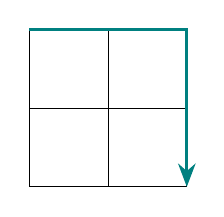
\begin{tikzpicture}
			\draw (0, 0) grid +(2,2);
			\draw[very thick, -Stealth, blue!50!green] (0, 2) -| (2, 0);
		\end{tikzpicture}
		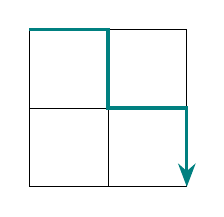
\begin{tikzpicture}
			\draw (0, 0) grid +(2,2);
			\draw[very thick, -Stealth, blue!50!green] (0, 2) -| (1, 1) -| (2,0);
		\end{tikzpicture}
		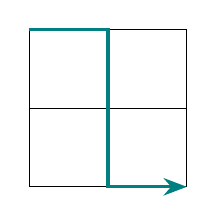
\begin{tikzpicture}
			\draw (0, 0) grid +(2,2);
			\draw[very thick, -Stealth, blue!50!green] (0, 2) -| (1, 0) -- (2, 0);
		\end{tikzpicture}

		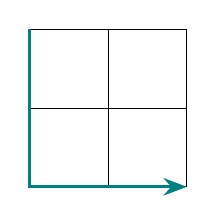
\begin{tikzpicture}
			\draw (0, 0) grid +(2,2);
			\draw[very thick, -Stealth, blue!50!green] (0, 2) |- (2, 0);
		\end{tikzpicture}
		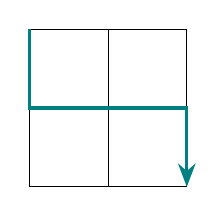
\begin{tikzpicture}
			\draw (0, 0) grid +(2,2);
			\draw[very thick, -Stealth, blue!50!green] (0, 2) |- (1, 1) -| (2,0);
		\end{tikzpicture}
		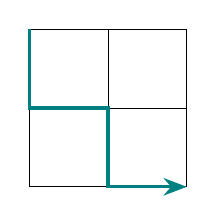
\begin{tikzpicture}
			\draw (0, 0) grid +(2,2);
			\draw[very thick, -Stealth, blue!50!green] (0, 2) |- (1, 1) |- (2,0);
		\end{tikzpicture}
	\end{center}

	在一个 $20 \times 20$ 的网格中,从左上角到右下角的路径,每次只能向右或向下移动一次。有多少条不同的路径从起点到终点?
\end{tcolorbox}

\subsection{算法}
这道题目要用到动态规划来解,最上边的第一个节点都依赖于其左边的节点有多少路径,与最上边相似,最左边的节点都依赖其上面的节点,在这里最上边与最左边的节点的路径数都为1。其他节点都依赖于其上方与左边的节点的数量,因此可以写成下面的伪代码:
\begin{algorithm}
	\caption{网格路径数}
	\begin{algorithmic}[1]
	\State 初始化一个 $(N+1) \times (N+1)$的矩阵,第1行全部为1,第一列也全部为1
	\State 遍历除第一行和第一列以外的节点,每个节点的值等于上方的值+左边的值
	\end{algorithmic}
\end{algorithm}


\subsection{答案}

\section{数字的数字和}\label{sec:problem16}
\subsection{问题描述}
\begin{tcolorbox}
2 的 15 次方是 32768,其数字和为 3 + 2 + 7 + 6 + 8 = 26。

计算 2 的 1000 次方的数字和是多少?
\end{tcolorbox}

\subsection{算法}
可以将字符串数字类中实现一个乘法,在乘法的基础上实现幂运算。然后还需要实现一个计算数字和的函数。

\subsection{答案}
1366

\section{数字文字计数}\label{sec:problem17}
\subsection{问题描述}
\begin{tcolorbox}
	如果将 1 到 5 写成英文单词,它们分别是:

	\begin{itemize}
		\forcsvlist{\item}{
			1 = \enquote{one},
			2 = \enquote{two},
			3 = \enquote{three},
			4 = \enquote{four},
			5 = \enquote{five},
		      }
	\end{itemize}
	这些单词的字母数量为 3、3、5、4 和 4。因此,1 到 5 的数字单词一共有
	$ 3 + 3 + 5 + 4 + 4 = 19 $
	个字母。

	从 1 到 1000(含 1000)中的每个数字用英文单词来表示,不计空格和连字符,总共有多少个字母?

	例如:
	342(three hundred and forty-two)包含 23 个字母。

	115(one hundred and fifteen)包含 20 个字母。

	注意:不计空格或连字符,\enquote{and} 是按规则包含在使用中的英文单词中。
\end{tcolorbox}

\subsection{算法}
\begin{enumerate}
	\item 准备数字到英文单词的映射表:我们需要将 1 到 19 的单词直接映射。对于整十数(20, 30, ...,
		90),也要单独映射。然后为\enquote{hundred}(100)和\enquote{thousand}(1000)定义规则。
	\item 分段处理数字:例如,对于 342,英文单词表示为 \textit{three hundred and forty-two}。我们可以将数字拆分为百位数、十位数、个位数,分别进行转换。
	\item 处理特殊情况:例如 100 到 999 之间的数字,需要注意添加 \enquote{and}。
	\item 统计字母数:统计所有数字转换成单词后的字母数量,不计空格和连字符。
\end{enumerate}

\subsection{答案}
21124

\section{标题}
\subsection{问题描述}
\begin{tcolorbox}
	给定一个三角形,从顶部到底部选择一条路径,使得路径上的数字总和最大。如下所示:

	\[
		\begin{aligned}
			  &   &                    & \textcolor{red}{3} &                    &   &   \\
			  &   & \textcolor{red}{7} &                    & 4                  &   &   \\
			  & 2 &                    & \textcolor{red}{4} &                    & 6 &   \\
			8 &   & 5                  &                    & \textcolor{red}{9} &   & 3
		\end{aligned}
	\]

	在这个例子中,最大的路径和为 23。请找到这个最大路径和。

	\begin{center}
		75\\
		95 64\\
		17 47 82\\
		18 35 87 10\\
		20 04 82 47 65\\
		19 01 23 75 03 34\\
		88 02 77 73 07 63 67\\
		99 65 04 28 06 16 70 92\\
		41 41 26 56 83 40 80 70 33\\
		41 48 72 33 47 32 37 16 94 29\\
		53 71 44 65 25 43 91 52 97 51 14\\
		70 11 33 28 77 73 17 78 39 68 17 57\\
		91 71 52 38 17 14 91 43 58 50 27 29 48\\
		63 66 04 68 89 53 67 30 73 16 69 87 40 31\\
		04 62 98 27 23 09 70 98 73 93 38 53 60 04 23\\
	\end{center}
\end{tcolorbox}

\subsection{算法}
这道题目用动态规划的方法来求解。

\subsection{答案}
1074

\section{标题}
\subsection{问题描述}
\begin{tcolorbox}
在1901年1月1日到2000年12月31日的这段时间内,有多少个月的1号是星期天?已知:
\begin{itemize}
    \item 1900年1月1日是星期一;
    \item 闰年规则为:如果年份能被4整除但不能被100整除,或者能被400整除,则该年为闰年;
    \item 每月天数:
    \begin{itemize}
        \item 31天:1月、3月、5月、7月、8月、10月、12月;
        \item 30天:4月、6月、9月、11月;
        \item 28天:2月,闰年为29天。
    \end{itemize}
\end{itemize}
\end{tcolorbox}

\subsection{算法}
先实现一个闰年判断的函数
\begin{algorithm}
	\caption{算法标题}
	\begin{algorithmic}[1]
		\If{$Y \mod 400 = 0$ or $(Y \mod 4 = 0$ and $Y \mod 100 \neq 0) $}
		\Return \textbf{true}
	\EndIf
	\end{algorithmic}
\end{algorithm}

\subsection{答案}

\section{阶乘数字和}\label{sec:problem20}
\subsection{问题描述}
\begin{tcolorbox}
求 $100!$ 的各位数字和。即:
\[
100! = 100 \times 99 \times \cdots \times 2 \times 1
\]
计算得到的阶乘结果后,求其各位数字的和。例如:
\[
10! = 10 \times 9 \times \cdots \times 1 = 3628800
\]
其各位数字之和为:
\[
3 + 6 + 2 + 8 + 8 + 0 + 0 = 27
\]
\end{tcolorbox}

\subsection{算法}
用前面实现的字符串数字类中添加个阶乘的算法。

\subsection{答案}
648

\section{亲和数之和}
\subsection{问题描述}
\begin{tcolorbox}
	定义 $d(n)$ 表示 $n$ 的所有真因数(即小于 $n$ 的除 $n$ 之外的除数)的和。

	如果 $d(a) = b$ 且 $d(b) = a$,并且 $a \neq b$,那么 $a$ 和 $b$ 被称为亲和数。例如,220 和 284 就是一对亲和数:

	\[
		d(220) = 1 + 2 + 4 + 5 + 10 + 11 + 20 + 22 + 44 + 55 + 110 = 284
	\]
	\[
		d(284) = 1 + 2 + 4 + 71 + 142 = 220
	\]

	求小于10000的所有亲和数的和。
\end{tcolorbox}

\subsection{算法}
\begin{enumerate}
	\item 编写函数 $d(n)$,计算 $n$ 的所有真因数的和。
	\item 对于每个小于10000的数字 $a$,计算 $b = d(a)$,如果 $d(b) = a$ 且 $a \neq b$,则 $a$ 和 $b$ 是亲和数。
	\item 注意避免重复计算。
\end{enumerate}

\subsection{答案}

\section{名字记分}\label{sec:problem22}
\subsection{问题描述}
\begin{tcolorbox}

给定一个超过五千个名字的文件,将这些名字按字母顺序排序。然后,对于每个名字,按以下步骤计算得分:

\begin{enumerate}
    \item 计算名字的字母值:将名字中每个字母的字母顺序($A=1, B=2, ..., Z=26$)相加。例如,$COLIN$ 的字母值为 $3 + 15 + 12 + 9 + 14 = 53$。
    \item 将名字的字母值乘以其在排序后的位置索引,得到名字的得分。例如,"COLIN" 在排序后是第938个名字,其得分为 $938 \times 53 = 49714$。
\end{enumerate}
\end{tcolorbox}

\subsection{算法}
\begin{enumerate}
    \item 读取文件并去除名字的引号。
    \item 按字母顺序对名字进行排序。
    \item 对于每个名字,计算其字母值,并乘以其在排序中的位置,计算名字得分。
    \item 将所有名字的得分相加,得到结果。
\end{enumerate}

\subsection{答案}
871198282

\section{非盈数之和}
\subsection{问题描述}
\begin{tcolorbox}
	如果一个数的真因数之和大于该数本身,则称该数为\textbf{盈数}。例如,$12$ 是最小的盈数,它的真因数之和为:
	\[
		1 + 2 + 3 + 4 + 6 = 16
	\]
	大于12。找出所有不能写成两个盈数之和的正整数,并求它们的总和。

	已知:所有大于28123的数字都可以写成两个盈数之和,因此我们只需考虑小于等于28123的数字。

\end{tcolorbox}

\subsection{算法}
\begin{enumerate}
	\item \textbf{判断盈数}:编写函数判断某个数是否为盈数。
	\item \textbf{生成盈数}:找出所有小于等于28123的盈数。
	\item \textbf{判断是否为两个盈数之和}:通过分解一个数字为两个部分,分别计算是否为盈数。
	\item \textbf{求和}:遍历所有小于等于28123的数字,计算那些不能表示为两个盈数之和的数字总和。
\end{enumerate}

\subsection{答案}
4179871

\section{字典序排列}\label{sec:problem24}
\subsection{问题描述}
\begin{tcolorbox}
排列是对象的一种有序排列。例如,3124 是数字 1、2、3 和 4 的一种可能的排列。如果所有排列都按数值或字母顺序列出,我们称之为字典序。数字 0、1 和 2 的字典序排列如下:

\begin{enumerate}
  \item 012
  \item 021
  \item 102
  \item 120
  \item 201
  \item 210
\end{enumerate}

请问数字 0、1、2、3、4、5、6、7、8 和 9 的第 1,000,000 个字典序排列是什么?
\end{tcolorbox}

\subsection{算法}
排列的算法是从数组的最右边开始搜索,如果找到一个元素,其左边(P)的值比自身小,再从左到右搜索一个比P大的值,则两个元素对调,然后对P右边的元素从小到大排序。

\subsection{答案}
2783915604

\section{第一个有1000位数的斐波那契数}\label{sec:problem25}
\subsection{问题描述}
\begin{tcolorbox}

斐波那契数列定义为:

\[
F_1 = 1, \quad F_2 = 1, \quad F_n = F_{n-1} + F_{n-2} \, \text{对} \, n \geq 3.
\]

求第一个有1000位的斐波那契数 \( F_n \) 的序号。
\end{tcolorbox}

\subsection{算法}
用之前实现的字符串数字类可以轻松解决这个问题。

\subsection{答案}
4782

\section{倒数的循环节}\label{sec:problem26}
\subsection{问题描述}
\begin{tcolorbox}
单位分数指的是分子为 1 的分数。分母为 2 到 10 的所有单位分数的小数部分如下所示:

\[
\frac{1}{2} = 0.5
\]
\[
\frac{1}{3} = 0.\overline{3}
\]
\[
\frac{1}{4} = 0.25
\]
\[
\frac{1}{5} = 0.2
\]
\[
\frac{1}{6} = 0.1\overline{6}
\]
\[
\frac{1}{7} = 0.\overline{142857}
\]
\[
\frac{1}{8} = 0.125
\]
\[
\frac{1}{9} = 0.\overline{1}
\]
\[
\frac{1}{10} = 0.1
\]

可以看出,\( \frac{1}{7} \) 有一个 6 位的循环节。

找出小于 1000 的所有单位分数中,小数部分循环节最长的分数的分母。
\end{tcolorbox}

\subsection{算法}
当分子小于分母的时候乘以10直到大于分母为止。

分子与分母求余,并将余数记录下来,如果出现相同的余数则视为循环出现。

\subsection{答案}

\section{二次表达式生成的素数}\label{sec:problem27}
\subsection{问题描述}
\begin{tcolorbox}
欧拉发现了这个著名的二次表达式:

\[
n^2 + n + 41
\]

对于 \( n = 0 \) 到 \( n = 39 \) 之间的每个 \( n \),该表达式生成了 40 个素数。然而,当 \( n = 40 \) 时,得到的 \( 40^2 + 40 + 41 = 1681 \) 并不是一个素数。该二次表达式生成了从 \( n = 0 \) 到 \( n = 39 \) 的连续素数。

发现了以下的二次表达式:

\[
n^2 - 79n + 1601
\]

对于 \( n = 0 \) 到 \( n = 79 \) 之间的每个 \( n \),该表达式生成了 80 个素数。这一表达式生成的连续素数的系数积为 \( -79 \) 和 1601,积为 \( -79 \times 1601 = -126479 \)。

考虑形如 \( n^2 + an + b \) 的二次表达式,其中 \( |a| < 1000 \) 且 \( |b| \leq 1000 \)。

找出系数 \( a \) 和 \( b \) 使得表达式 \( n^2 + an + b \) 对于从 \( n = 0 \) 开始的连续整数 \( n \) 生成最多的素数,计算出此时 \( a \) 和 \( b \) 的乘积。

\end{tcolorbox}

\subsection{算法}
最简单粗暴的方法是直接两遍循环,但是这种方法的消耗是指数级增长的。我们可以对暴力循环进行一些优化。

\begin{itemize}
  \item 首先,我们来考虑 \( b \),当 \( n = 0 \),二项式的值为 \( b \),所以 \( b \)必须为素数才行;
  \item \( a \)的值比较自由,但是也有可以考虑的点,比如当 \( n = 1 \)时,二项式的值为 \( 1 + a + b
    \),除了值等于2的情况,其他情况下, \( a \)和 \( b \)的奇偶性必须是相同的。但是因为 \( b \)必须为素数,所以也排除了
    \( n = 1 \)时二项式的值为2的情况,所以 \( a \)和 \( b \)同奇或者同偶。
\end{itemize}

\subsection{答案}
-59231

\section{螺旋矩阵对角线之和}
\subsection{问题描述}
\begin{tcolorbox}

	从数字1开始,按顺时针顺序依次将连续的奇数排列成一个边长为 5 的螺旋矩阵如下所示:

	\[
		\begin{matrix}
			\red{21} & 22      & 23      & 24      & \red{25} \\
			20       & \red{7} & 8       & \red{9} & 10       \\
			19       & 6       & \red{1} & 2       & 11       \\
			18       & \red{5} & 4       & \red{3} & 12       \\
			\red{17} & 16      & 15      & 14      & \red{13}
		\end{matrix}
	\]

	可以看到,该矩阵对角线上的数字之和为 101。

	考虑更大的边长为 1001 的螺旋矩阵,求该矩阵对角线上的数字之和。
\end{tcolorbox}

\subsection{算法}
对角线数字的生成方法为:
\begin{itemize}
	\item 从1开始,第二层矩阵的对角线四个角点分别加2;
	\item 下一层的矩阵的步长要加2;
\end{itemize}

\subsection{答案}

\section{不同幂次之和}
\subsection{问题描述}
\begin{tcolorbox}
考虑所有形如 \( a^b \) 的幂次组合,其中 \( 2 \leq a \leq 5 \) 且 \( 2 \leq b \leq 5 \):

\[
2^2 = 4, \quad 2^3 = 8, \quad 2^4 = 16, \quad 2^5 = 32
\]
\[
3^2 = 9, \quad 3^3 = 27, \quad 3^4 = 81, \quad 3^5 = 243
\]
\[
4^2 = 16, \quad 4^3 = 64, \quad 4^4 = 256, \quad 4^5 = 1024
\]
\[
5^2 = 25, \quad 5^3 = 125, \quad 5^4 = 625, \quad 5^5 = 3125
\]

如果将这些幂次组合按大小排列并去除重复的项,我们得到如下的序列:

\[
4, 8, 9, 16, 25, 27, 32, 64, 81, 125, 243, 256, 625, 1024, 3125
\]

这些组合一共有 15 项。

考虑所有形如 \( a^b \) 的幂次组合,其中 \( 2 \leq a \leq 100 \) 且 \( 2 \leq b \leq 100 \),求出这些幂次组合中不同的项有多少个。

\end{tcolorbox}

\subsection{算法}
这个问题的最主要问题是大数的处理,有了之前的字符串数字,解决这个问题就容易多了。

\subsection{答案}
9183

\section{数字的第五次幂}\label{sec:problem30}
\subsection{问题描述}
\begin{tcolorbox}

令人惊讶的是,只有三个数字可以写成它们各位数字的第四次幂之和:

\[
1634 = 1^4 + 6^4 + 3^4 + 4^4
\]

\[
8208 = 8^4 + 2^4 + 0^4 + 8^4
\]

\[
9474 = 9^4 + 4^4 + 7^4 + 4^4
\]

由于 $1 = 1^4$ 不是一个和,所以不包括在内。

这些数字的和是:

\[
1634 + 8208 + 9474 = 19316
\]

找出所有可以写成它们各位数字的第五次幂之和的数字的总和。
\end{tcolorbox}

\subsection{算法}
这道题实现起来并不难,主要是考虑判断的边界问题,这里的判断是到6位数为止,因为6位数最大为\num{999999},其数字的5次方之和为\num{354294},已经小于\num{999999}。而如果增加到7位数,最小的7位数是\num{1000000},而即使是\num{9999999}的数字5次方之和也只有\num{413343}。

另外一个可以优化的地方是可以将0--9所有数字的5次方计算出来,后面直接从数组中读取可以避免重复计算的问题。

\subsection{答案}
443839

\section{硬币组合}
\subsection{问题描述}
\begin{tcolorbox}

	在英国,硬币有1p、2p、5p、10p、20p、50p、£1 和 £2 的面额。计算有多少种不同的方式可以用这些硬币组合成总额为 £2?
\end{tcolorbox}

\subsection{算法}
这种问题用动态规划解决是最佳方案。用一个数组\texttt{dp}来记录每增加一种硬币方案数量的变化。

主要实现思路如下:
\begin{enumerate}
	\item 初始化一个 \( 200 + 1 \)长度的 \( dp \)数组, \( dp[0] = 1 \);
	\item 遍历所有币种,每种币种从其币值 \( m \)开始 \( dp[x] += dp[x - m] \)
\end{enumerate}

\subsection{答案}

\section{全数字乘积}\label{sec:problem32}
\subsection{问题描述}
\begin{tcolorbox}
	我们称一个 $n$ 位数字为“全数字”的,如果它恰好使用了从 1 到 $n$ 的所有数字一次;例如,5 位数字 $15234$ 就是 1 到 5 的全数字。

	数字 $7254$ 是不寻常的,因为等式 $39 \times 186 = 7254$ 中的乘数、乘数和乘积都是 1 到 9 的全数字。

	找出所有被乘数/乘数/乘积等式可以写成 1 到 9 的全数字的所有乘积的和。

	提示:有些乘积可以通过不止一种方式获得,因此确保在你的总和中只包含一次。
\end{tcolorbox}

\subsection{算法}
将1-9这几个数字组成的字符串用\texttt{next\_permutation},然后对字符串进行分割。一共只有两种方式, \( (1,4,4)\) 和\( (2,3,4)
\),分割之后检查乘法是否成立。因为有可能会有重复的乘积,所以用\texttt{unordered\_set}来存储结果。

\subsection{答案}
$45228$

\section{数字抵消分数}
\subsection{问题描述}
\begin{tcolorbox}
	分数 \( \frac{49}{98} \) 是一个有趣的分数,因为一个没有经验的数学家在尝试简化它时可能会错误地认为 \( \frac{49}{98} = \frac{4}{8} \),这是正确的,是通过取消数字 9 得到的。

	我们将考虑像 \( \frac{30}{50} = \frac{3}{5} \) 这样的分数作为平凡的例子。

	在数值小于1且分子分母都包含两位数的分数中,恰好有四个非平凡的例子。

	如果这四个分数的乘积以最简形式给出,求分母的值。
\end{tcolorbox}

\subsection{算法}
根据要求分子必须比分母小,所以经过简单的推算,可以抵消的必须要错位,就是抵消分子的10位数的话,分母上就需要是个位。

假设 \( \frac{ax}{bx} = \frac{a}{b} \), 则有 \(  (10a + x) b = (10b + x) a \),进一步化简可以得到 \( a = b
\),这样分子就等于分母,与题目中分数的值要小于1不符。同样也可以证明不能是分子分母的10位相同。

\subsection{答案}
\( 100 \)

\section{数字阶乘和}
\subsection{问题描述}
\begin{tcolorbox}

	由于 $1! + 2! + 145! = 145$,因此,145 是一个特殊的数。请找出所有满足以下条件的数的和:
	\begin{itemize}
		\item 这些数等于它们各个数字阶乘的和。
	\end{itemize}

	\textbf{数学公式}:

	一个数 $n$ 被称为特殊数,如果
	\[
		n = \sum_{i=1}^{k} d_i!
	\]
	其中 $d_i$ 是 $n$ 的每一位数字,$k$ 是数字的位数。

    注意,1和2只有一个数字不被计算在内。
\end{tcolorbox}

\subsection{算法}
在最开始的时候数字的阶乘和增长很快, \( 9! = 362880
\),但是数字随着位数的增长速度变得更快,\num{999999}的数字阶乘和为\num{2177280},\num{9999999}为\num{2540160},后面数字位数增长引发值增大的速度远远超过了数字阶乘和,所以只需要判断到7位数就OK了。

\subsection{答案}
40730

\section{环形素数}
\subsection{问题描述}
\begin{tcolorbox}

素数 \( p \) 称为环形素数,如果其所有旋转都是素数。例如,13 是一个环形素数,因为它的旋转 13 和 31 都是素数。

考虑所有小于 1,000,000 的环形素数的总数。
\end{tcolorbox}

\subsection{算法}
这道题只需要解决如何构造环形数的问题即可,结合之前的素数判断的方法即可解决此问题。

构造环形数只需要计算出数$n$的位数$p$,将数 \( n \)分成两部分, \( p - 1 \)位 \( b \)和最后一个数字 \( e \),新的生成数即为:
\begin{equation*}
 10^pe + b
\end{equation*}
将这个过程循环 \( p \)次即可完成变化。


\subsection{答案}

\section{十进制和二进制回文数}
\subsection{问题描述}
\begin{tcolorbox}

回文数是左到右和从右到左读起来都一样的数。例如,585 是一个回文数。

在十进制和二进制表示下,某些回文数同时也是回文数。例如,585 是一个回文数(十进制),在二进制表示下也是一个回文数:1001001001。

找到所有小于 1,000,000 的数字中,既是十进制回文数又是二进制回文数的数字之和。
\end{tcolorbox}

\subsection{算法}
回文数的判定之前已经写过,所以只需要实现二进制回文数的判定,这个可以用回文数判定的算法,将基数变为2即可。


\subsection{答案}

\section{可截素数}\label{sec:problem37}
\subsection{问题描述}
\begin{tcolorbox}

可截素数指的是:从左到右和从右到左逐位截去数字后,剩下的所有数字仍然是素数。例如,3797 是一个可截素数:

\begin{itemize}
    \item 从左到右依次截去:3797、797、97、7 都是素数;
    \item 从右到左依次截去:3797、379、37、3 也是素数。
\end{itemize}

只考虑两位数及以上的素数,求所有这样的素数之和(一共只有11个)。

\end{tcolorbox}

\subsection{算法}

依次用 \( 10, 100, \cdots \) 来对要判断的质数 \( n \)取余,并依次判断余数是不是质数。

\subsection{答案}
748317

\section{全数字乘积}\label{sec:problem38}
\subsection{问题描述}
\begin{tcolorbox}

将 192 与 1、2 和 3 分别相乘:

\[
192 \times 1 = 192
\]
\[
192 \times 2 = 384
\]
\[
192 \times 3 = 576
\]

将这些乘积连接起来,我们得到一个 1 到 9 的全数字(192384576)。我们称 192384576 为 192 和 (1,2,3) 的连接乘积。

同样,对于 9 和 (1,2,3,4,5),我们可以得到全数字 918273645,这是一个 1 到 9 的全数字。

所求是能通过某个整数和 (1,2,...) 的倍数产生的最大全数字 1 到 9 的连接乘积。该整数不能有重复的数字,且必须包含每个数字恰好一次。
\end{tcolorbox}

\subsection{算法}
对于每一个 \( 123456789 \)的排列,测试以下几种情况:
\begin{enumerate}
	\item 将第1位数依次乘以23456789
	\item 取前面2位数
	\item 取前面3位数
	\item 取前面4位数
\end{enumerate}
5位数不用再考查,因为加起来会超过10位数。

因为是求最大的连接乘积,所以可以从最大的987654321开始用prev\_permutation函数。

\subsection{答案}
932718654

\section{整数边长直角三角形}
\subsection{问题描述}
\begin{tcolorbox}

	如果一个直角三角形的边长为整数,则其周长 \( p \) 是边长的和。对于周长 \( p = 120 \),有三个不同的解:

	\[
		(20, 48, 52),\ (24, 45, 51),\ (30, 40, 50)
	\]

	对于给定的 \( p \leq 1000 \),找出具有最多解的 \( p \) 值。
\end{tcolorbox}

\subsection{算法}
斜边小于两个直角边之和。

\subsection{答案}

\section{Champernowne 常数}
\subsection{问题描述}
\begin{tcolorbox}

	Champernowne 常数是通过将正整数序列连接起来构成的一个无限小数。例如:

	\[
		0.12345678910\red{1}112131415161718192021\ldots
	\]

	这个小数包含了所有的正整数数字,依次排列。

	给定 Champernowne 常数的第 \( n \) 位是指小数中第 \( n \) 位的数字。

	求出下列位置上的数字的乘积:

	\[
		d_1 \times d_{10} \times d_{100} \times d_{1000} \times d_{10000} \times d_{100000} \times d_{1000000}
	\]

	其中 \( d_n \) 表示 Champernowne 常数中第 \( n \) 位的数字。
\end{tcolorbox}

\subsection{算法}
\begin{enumerate}
	\item 计算目标所在的区域,将$ n $ 循环减去 \( 9, 90 \times 2, 900 \times 3 \)直到 \( n \) 小于当前数字宽带的数字的总和。
	\item 将 \( n  - 1\) 与当前的数字宽度求余,再加之前的所有数字即得到第 \( n \)位数对应的数 \( P \)
	\item 计算目标在 	\( P \)上的索引号,然后将其取出。
\end{enumerate}

\subsection{答案}
210

\section{全数字素}
\subsection{问题描述}
\begin{tcolorbox}
一个 $n$ 位全数字数是指包含数字 $1$ 到 $n$ 中所有数字的排列且没有重复的数。例如,$2143$ 是一个 4 位全数字数,并且它恰好是一个素数。

求最大的全数字素数。
\end{tcolorbox}

\subsection{算法}
9位数和8位数的全数字之和分别是45和36,均是3的倍数,所以不可能是素数。可以从7654321开始,判断是不是素数,如果不是,再用perv\_permutation来生成一个排列,直到找到目标为止。

\subsection{答案}
7652413

\section{编码三角形数}
\subsection{问题描述}
\begin{tcolorbox}
	三角形数的生成公式为 $T_n = \frac{n(n+1)}{2}$,它的前十项是:

	\begin{equation*}
		1 , 3 , 6 , 10 , 15 , 21 , 28 , 36 , 45 , 55 , \cdots
	\end{equation*}
	给定一个单词的字母值,假设 $A=1, B=2, ..., Z=26$,则单词的字母值为所有字母对应数值的和。例如,单词 "SKY" 的字母值为
	$19 + 11 + 25 = 55$,它恰好是一个三角形数。

	在提供的\href{https://projecteuler.net/resources/documents/0042_words.txt}{文本文件}中包含了一系列单词,计算出其中有多少个单词的字母值是三角形数。
\end{tcolorbox}
\subsection{算法}
\begin{enumerate}
	\item 读取文件中的名字到数组
	\item 根据名字最大长度并假设每个字母都是 $Z$,计算出最大的分数
	\item 用三角形数公式生成能够覆盖最大名字分数的所有三角形数
	\item 用每个名字的分法在生成的三角形数中查找
\end{enumerate}

\subsection{答案}
162

\section{全数字的部分整除性}\label{sec:problem43}
\subsection{问题描述}
\begin{tcolorbox}
	将0到9这十个数字以某种排列组合的形式组成一个10位数,称为全数字数。例如,1406357289 是一个全数字数。

	假设 \( d_1 \) 表示第一个数字,\( d_2 \) 表示第二个数字,依此类推。我们定义如下特性:

	\begin{itemize}
		\item \( d_2d_3d_4 \) 能被 2 整除
		\item \( d_3d_4d_5 \) 能被 3 整除
		\item \( d_4d_5d_6 \) 能被 5 整除
		\item \( d_5d_6d_7 \) 能被 7 整除
		\item \( d_6d_7d_8 \) 能被 11 整除
		\item \( d_7d_8d_9 \) 能被 13 整除
		\item \( d_8d_9d_{10} \) 能被 17 整除
	\end{itemize}

	找到所有满足上述特性的全数字数,并求它们的和。

\end{tcolorbox}

\subsection{算法}
用 \( 0123456789 \)的排列变化来逐项进行判断,但是因为0不能放在首位,所以可以从 \( 1023456789 \)开始。

这种算法要计算出所有的排列,其实效率并不高,但是容易理解。

可以通过剪枝算法逐渐构造出整个10位的全数字数,因为不符合整除的条件的分枝被剪除了,所以避免了很多不必要的运算。

\subsection{答案}
16695334890

\section{五边形数}\label{sec:problem44}
\subsection{问题描述}
\begin{tcolorbox}
	五边形数由公式 $P_n = \dfrac{n(3n-1)}{2}$ 给出。前十个五边形数是:

	\[
		1, 5, 12, 22, 35, 51, 70, 92, 117, 145, \dots
	\]

	可以看出,$P_4 + P_7 = 22 + 70 = 92 = P_8$,但是它们的差 $70 - 22 = 48$ 不是五边形数。

	找出满足条件的五边形数对 $P_j$ 和 $P_k$,使得它们的和与差均为五边形数,并且 $D = |P_k - P_j|$ 的值最小。
\end{tcolorbox}

\subsection{算法}
将产生的五边形数顺序排列,然后将最后一个五边形数与之前的所有数计算差与和,并判定差与和是否为五边形数。

\subsection{答案}
5482660

\section{复合多边形数}
\subsection{问题描述}
\begin{tcolorbox}
	三角形数、五边形数和六边形数由以下公式给出:

	\[
		T_n = \frac{n(n + 1)}{2}
	\]
	\[
		P_n = \frac{n(3n - 1)}{2}
	\]
	\[
		H_n = n(2n - 1)
	\]

	可以发现, $ T_{285} = P_{165} = H_{143} =40755 $。

	找出下一个既是三角形数、五边形数、也是六边形数的数。

\end{tcolorbox}

\subsection{算法}
可以从 $ H_{144}$开始查找,用三角形数和五边形数的判断函数。

\begin{align*}
	T_n        & = \frac{n(n+1)}{2}                      \\
	2T_n       & = n^2 + n                               \\
	8T_n       & = 4n^2 + 4n + 1 - 1                     \\
	(2n + 1)^2 & = 8T_n + 1                              \\
	n          & = \frac{\sqrt{8T_n + 1} - 1}{2} \tag{1}
\end{align*}

\begin{align*}
	P_n        & = \frac{n(3n - 1)}{2}                    \\
	2P_n       & = 3n^2 - n                               \\
	24P_n      & = 36n^2 - 12n + 1 - 1                    \\
	(6n - 1)^2 & = 24P_n + 1                              \\
	n          & = \frac{\sqrt{24P_n + 1} + 1}{6} \tag{2}
\end{align*}
六边形的判断其实这道题里面用不到,不过这里还是列一下算法:
\begin{align*}
	H_n        & = n(2n - 1)                             \\
	H_n        & = 2n^2 - n                              \\
	8H_n       & = 16n^2 - 8n + 1 - 1                    \\
	(4n - 1)^2 & = 8H_n + 1                              \\
	n          & = \frac{\sqrt{8H_n + 1} + 1}{4} \tag{3}
\end{align*}
\subsection{答案}
1533776805

\section{哥德巴赫的其他猜想}
\subsection{问题描述}
\begin{tcolorbox}
克里斯蒂安·哥德巴赫曾经提出了一个猜想:任何一个大于2的奇合数都可以写成一个素数加上一个平方数的两倍,即:

\[
n = p + 2 \times k^2
\]

其中,\( n \) 是奇合数,\( p \) 是素数,\( k \) 是一个正整数。

这个猜想后来被证明是错误的。也就是说,存在一个奇合数无法用上述方式表示。

找出最小的那个不能被写成素数加上两倍平方数的奇合数。
\end{tcolorbox}

\subsection{算法}


\subsection{答案}

\section{不同质因数}
\subsection{问题描述}
\begin{tcolorbox}
找出第一个有四个不同质因数的连续整数。换句话说,每个数都有恰好四个不同的素因数。 

例如,第一个有两个不同质因数的连续整数是:

\[
14 = 2 \times 7
\]
\[
15 = 3 \times 5
\]

现在,找出第一个有四个不同质因数的连续四个整数。

\end{tcolorbox}

\subsection{算法}


\subsection{答案}

\section{标题}
\subsection{自幂之和}
\begin{tcolorbox}

计算以下表达式的最后十位数:

\[
1^1 + 2^2 + 3^3 + \cdots + 1000^{1000}
\]


\end{tcolorbox}

\subsection{算法}


\subsection{答案}

\section{素数排列}\label{sec:problem49}
\subsection{问题描述}
\begin{tcolorbox}
考虑由三个不同的素数组成的等差数列,这三个素数由相同的数字重排组成。比如,1487、4817 和 8147 就是这样的一个序列。

这个序列有一个显著的性质:1487、4817 和 8147 是三个 4 位数,并且每一个都是素数。更有趣的是,这三个数字的差值相同:4817 - 1487 = 3330,8147 - 4817 = 3330。

还有一个 4 位数的递增序列也满足这个性质,但它并不是将 1487、4817 和 8147 简单重排所得。找到这个序列,并将其三个项连接起来形成 12 位数。这个 12 位数是多少?
\end{tcolorbox}

\subsection{算法}
生成1万以内的素数数组,从1000开始验证,如果是素数的情况下,再进行一次内循环,检查数字是否为素数,与外循环的数是否数字相同。然后计算出第三个数,需要满足的条件的是第三个数要小于10000,并且是素数,而且与外循环或者内循环的数字相同。

\subsection{答案}
296962999629

\section{连续素数和}\label{sec:problem50}
\subsection{问题描述}
\begin{tcolorbox}
	素数41可以写成6个连续素数之和:

	\[
		41 = 2 + 3 + 5 + 7 + 11 + 13
	\]

	这也是一个素数。

	同样地,100以下最长的连续素数和是953,由21个连续素数相加得到:
	\begin{multline*}
		953 = 7 + 11 + 13 + 17 + 19 + 23 + 29 + 31 + 37 + 41 + 43 + 47 + 53 + 59 + 61\\ + 67 + 71 + 73 + 79 + 83
	\end{multline*}

	找出小于一百万的素数中,可以写成连续素数和的最长序列的素数。

\end{tcolorbox}

\subsection{算法}
用欧拉筛生成素数数组,从2开始连续加,找到不超过1百万的最大长度,如果在这个长度找不到,就长度减一,就这样循环搜索,直到找到答案。

\subsection{答案}
997651

\section{素数数字替换}
\subsection{问题描述}
\begin{tcolorbox}
通过将素数中的某些(不一定连续的重复数字)位替换成相同的数字,可以生成一个素数家族。例如,位于56003的第三位和第四位替换成相同的数字,我们可以得到以下十个数:

\[
56003, 56113, 56223, 56333, 56443, 56553, 56663, 56773, 56883, 56993
\]

其中,满足素数条件的有7个:56003, 56113, 56333, 56443, 56663, 56773 和 56993。

在这些素数中,56003是第一个在这种情况下可以产生一个七素数家族的成员。

找出满足这个性质的八素数家族的最小素数。
\end{tcolorbox}

\subsection{算法}


\subsection{答案}

\section{排列倍数}
\subsection{问题描述}
\begin{tcolorbox}
可以看出,数字 125874 与其两倍 251748 含有完全相同的数字,但顺序不同。

找出最小的正整数 $x$,使得 $2x, 3x, 4x, 5x, 6x$ 含有完全相同的数字。
\end{tcolorbox}

\subsection{算法}


\subsection{答案}

\section{组合数计算}
\subsection{问题描述}
\begin{tcolorbox}
已知有 10 种从 5 个数 12345 中选出 3 个数的方法:

\[ 
123, 124, 125, 134, 135, 145, 234, 235, 245, 345 
\]

在组合数学中,我们使用以下符号来表示组合数:

\[
\binom{5}{3} = 10
\]

一般来说,组合数公式为:

\[
\binom{n}{r} = \frac{n!}{r!(n - r)!}
\]

其中,\(r \leq n\),且 \(n! = n \times (n-1) \times \cdots \times 1\),且 \(0! = 1\)。

当 \(n = 23\) 时,组合数首次超过 100 万:

\[
\binom{23}{10} = 1144066
\]

问题:在 \( 1 \leq n \leq 100 \) 的范围内,有多少个不一定互不相同的组合数 \( \binom{n}{r} \) 的值大于一百万?

\end{tcolorbox}

\subsection{算法}
这道题当然可以用设计的大数来解决,但是如果采取一些优化算法还是可以避免溢出的。

分子与分母每一次计算时都用最小公倍数来减小。

第二种是用combination的另外一个递推公式:
\begin{equation*}
\binom{n}{r}=\binom{n-1}{r-1}+\binom{n-1}{r}
\end{equation*}
这个方法更高效和通用,也不会有溢出的风险。
\subsection{答案}
4075

\end{document}
